
\chapter{L'informazione e il web semantico (*)}

	\section{La torre di Babele del web}
	
		\subsection{Un esempio di problema informativo}
			Con l'espansione del web si sperimentano i primi bot cattura informazione. Uno di questi sistemi creato dal MIT permetteva un acquisto in pochi passi. Una \emph{query} famosa fu "manda una rosa alla mia ragazza", il bot trovò il prodotto desiderato e anche ne trovò un altro che corrispondeva a tutt'altro.
			Lo stesso capitò alla RIA (l'equivalente della SIAE) con un proprio bot che scovò una canzone piratata del cantante Usher ma che in realtà si rivelò una canzone completamente diversa, creata a scopo educativo dal professor Peter Usher.
			Molti investimenti sono stati fatti e ad oggi i bot sfruttano i tipi semantici, comprendendo. Vediamo come:
		
		\subsection{Evoluzione}
			Ma se al posto dell'Html avremmo informazione strutturata? Così facendo potremmo rimuovere le  ambiguità e le macchine potrebbero "capire" le informazioni del web. Uno strumento per fare questo può essere l'XML, semplice e flessibile, creato proprio per la necessità di strutturazione dei dati. Purtroppo proprio da questi stessi vantaggi nacquero molti dialetti che resero impossibile l'aggregazione. L'XML uscito fallimentare dall'\emph{open world} portò quindi alla necessità di creare un nuovo livello superiore che permettesse l'aggregazione e un nuovo strumento che lo descrivesse: l'RDF. Vediamo i vantaggi rispetto l'XML:
			\begin{itemize}
				\item le informazioni mappano su un modello non ambiguo. In ogni modello RDF si può riconoscere quali bit rappresentano la semantica e quali la sintassi di contorno.
				\item l'RDF è parte del web semantico.
			\end{itemize}
			L'RDF è quello strumento che mancava per rendere possibile l'aggregazione dell'informazione e il ragionamento automatico su di essa.
		
	\section{Il web semantico}
	
		\subsection{Babel Fish: l'RDF}
			Babel Fish è un traduttore istantaneo biologico descritto all'interno del libro \emph{Guida Galattica per gli Autostoppisti} di Douglas Adams. Il modello RDF (\emph{Resource Description Framework} può certamente interpretare questo ruolo di traduttore dal web che conosciamo a quello semantico come vediamo nella figura ~\ref{fig:LInformazioneEIlWebSemantico-WebSemantico}.
			
			\begin{figure}
				\centering
				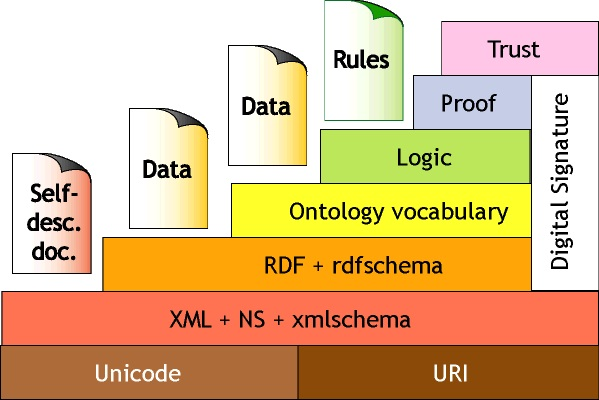
\includegraphics[scale=0.5]{images/LInformazioneEIlWebSemantico-WebSemantico1}
				\caption{Il web semantico - \emph{Layer} che compongono l'informazione}
				\label{fig:LInformazioneEIlWebSemantico-WebSemantico}
			\end{figure}			
			
			\subsubsection{Il modello RDF}
				Il modello RDF è un \emph{framework} comune che descrive metadati, relazioni e concetti garantendo l'interoperabilità tra essi. Si basa sulla grammatica di base:
				\begin{quote}
					$\langle$ soggetto - predicato - complemento oggetto $\rangle$
				\end{quote}
				Questi tre elementi possono contenere due diversi tipi di dati:
					\begin{itemize}
						\item URI,
						\item Stringhe letterali;
					\end{itemize}
				che compongono la struttura linguistica e logica più semplice. Questa struttura può essere visualizzata come un grafo ~\ref{fig:LInformazioneEIlWebSemantico-RDF1}.
				
				\begin{figure}
				\centering
					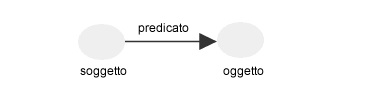
\includegraphics[scale=0.8]{images/LInformazioneEIlWebSemantico-RDF1}
					\caption{Il web semantico - Grammatica di base}
					\label{fig:LInformazioneEIlWebSemantico-RDF1}
				\end{figure}
				
				L'RDF può essere rappresentato in due modi differenti:
				\begin{description}
					\item[dialetto XML] usando la struttura XML per alzare la complessità e arricchire il significato.
					\item[N-triple] usando le triplette soggetto-predicato-verbo.
				\end{description}
				Esempio di tripletta della frase \emph{"il cielo è blu"} contenente due stringhe:
				\begin{quote}
				\begin{verbatim}
					<rdf:Description rdf:about='cielo'>
					<v:essere>blu</v:essere>
					</rdf:Description>
				\end{verbatim}
				\end{quote}
				
				L'RDF è un linguaggio separato dal web comune, per integrarlo si è ricorso ad una versione XHTML2: l'RDFa che aggiunge gli attributi \emph{about} (il soggetto) e \emph{property} (il verbo), il contenuto è il complemento oggetto.
				
			
			\subsubsection{Funzionalità e proprietà di RDF}
			
				\begin{description}
					\item[Aggregazione:] l'unione di due grafi di conoscenza è un grafo creato tramite collegamenti automatici dei nomi del web (URI). Questa è la proprietà più importante e che decreta il successo di RDF rispetto ai dialetti XML. 
					\item[Contenitori:] concetti logici di AND e OR.
					\item[Variabili:] oggetti logici non specificati.
					\item[Monotonicità:] preso un grafo, se l'informazione espressa in esso supponiamo sia vera allora tutti i sottografi sono veri.
					\item[Reificazione:] garantisce la monotonicità, riduce ad un oggetto (\emph{"cosifica"} cit.) una asserzione. Per esempio nella frase \emph{"Gromit dice che 'la luna è di formaggio'"}, la frase nel sottolivello \emph{"la luna è di formaggio"} è in realtà un'altra frase che grazie al processo di reificazione diventa un oggetto, per cui, anche se non sappiamo sia vero ciò non influisce nella veridicità della prima frase. Grazie a ciò abbiamo anche una diversificazione di livelli.
				\end{description}
				
				Gli oggetti devono essere anche classificati garantendo un costo computazionale minimo. Abbiamo bisogno di un \textbf{sistema di classificazione dell'informazione}: un'ontologia che contenga tipi semantici. Mentre i \textbf{tipi} danno il formato sintattico dell'oggetto, i \textbf{tipi semantici} gli danno il significato astraendo la rappresentazione sintattica.
				
			\subsubsection{I tipi semantici}
				Abbiamo visto con il caso \emph{"Usher vs Peter Usher"} che nel web mancano i tipi semantici. I tipi semantici possono essere astratti come classi. Un insieme di classi forma un'ontologia. Un'ontologia è costituita da:
				\begin{description}
					\item[Etichette:] rappresentanti caratteristiche informative (possono essere più di una per oggetto).
					\item[Struttura:] rappresentante la gerarchia di tutte le classi. Più una struttura è ricca e più l'ontologia mi permette di espandere le cose e la comprensione di esse. È grazie alla struttura che è possibile fare \textbf{controlli di integrità semantica} e \textbf{ragionamenti}.
				\end{description}
				
			\subsubsection{Caratteristiche di RDF Schema}
				L'RDF offre uno schema con una struttura informativa fatta di:
				\begin{itemize}
					\item \emph{Class};
					\item \emph{subClassOf};
					\item \emph{individual}.
				\end{itemize}
				Questo per gli oggetti mentre per i verbi abbiamo a disposizione:
				\begin{itemize}
					\item \emph{Property}; (la relazione, il verbo)
					\item \emph{subPropertyOf};
					\item \emph{Domain};
					\item \emph{range}. (dove la proprietà è applicata)
				\end{itemize}
				Grazie all'RDF Schema, quindi, possiamo \textbf{categorizzare l'informazione}.

			\subsubsection{Oltre l'RDF Schema}
				Abbiamo fissato delle regole semantiche ma siamo ancora al livello base delle ontologie (stato tassonomie). SI può fare molto di più: l'RDF permette l'aggregazione automatica attraverso l'URI. Ma gli URI presentano problemi di ambiguità.
			
		\subsection{L'architettura del web (Tim Berners-Lee)}
			Tim Berners-Lee prevedeva già questo alla nascita del web e infatti il web è nato seguendo questi assiomi:
			\begin{itemize}
				\item [0a)] A qualsiasi risorsa dovunque sia, essa può avere un nome. (\emph{assioma di universalità})
				\item [0b)] Ogni cosa di significato dovrebbe avere un URI. (\emph{assioma di universalità 2})
				\item [1)] Non importa a chi o dove specifichi un URI, ma che abbia sempre lo stesso significato. (\emph{global scope})
			\end{itemize}
			
			\subsubsection{Dare un nome ad ogni cosa: il problema degli URI}
				Trovare un nome (web) non è banale:
				\begin{description}
					\item[URI \emph{variant problem}:] esistono molte varianti per o stesso concetto.
					\item[URI \emph{variant law}:] l'utilità decresce esponenzialmente con il numero di varianti (legge della varianza degli URI). Più un nome ha diversi significati più questo perde valore.
					\item[URI \emph{variant size}:] un URI può acquisire diversi significati in base al dominio di interesse. "Problema \emph{big red barn}" cit. (se un bambino indica una mucca illustrata in un libro, ciò che indica è "una mucca" o "un libro"? Esistono livelli diversi).
				\end{description}
				
				Quanti studiosi di web semantico ci vogliono per avvitare una lampadina? 1 per avvitarla e gli altri 9 per mettersi d'accordo su che cos'è una lampadina.
				
			
			\subsubsection{La soluzione}
				La soluzione a questo inghippo è aggiungere più informazione. Abbiamo bisogno di maggiore informazione, un nuovo \emph{layer}: lo strato ontologico e un linguaggio ontologico.
		
		\subsection{Strato ontologico: OWL}
			Il supporto di base fornito da RDF Schema è stato quindi esteso con lo strato ontologico. Questo strato è descritto attraverso il linguaggio OWL (\emph{Web Ontology Language}) che si occupa di collegare e relazionare i vocaboli dando ad ognuno il proprio dominio d'interesse (la propria ontologia appunto).
		
			\subsubsection{Caratteristiche di OWL}
			
				L'(in)uguaglianza di OWL:	
					\begin{description}
						\item[EquivaleClass:]
						\item[equivalentProerty]
						\item[sakIndividualeAS]
						\item[differentFrom:]
						\item[allDifferent]
						\item[SameIndividualAs]
					\end{description}
					
				altre caratteristiche:
				
					\begin{itemize}
						\item inverseOf
						\item transitiveProperty
						\item simmetricProperty
						\item inverseFunctionalProperty
					\end{itemize}
					
			\subsubsection{Proprietà di OWL}
				
			\subsubsection{Il problema: ragionarci}
			
			
		\subsection{SPARQL}
		
			\subsubsection{Modellazione con SPARQL}		
				
				Vocabolari più famosi:
				\begin{description}
					\item[DC: Dublic Core]
					\item[FOAF: Friend Of A Friend]
				\end{description}		
		
		\subsection{Un problema di complessità (*)}
		
			La gerarchia dei problemi è:
			\[
				NL \subset P \subset NP \subset PSPACE \subset EXPTIME \subset EXPSPACE
			\]
			
			\subsubsection{La soluzione di SPARQL}
			
			\subsubsection{La soluzione di OWL}
				Lo strato che offre di più con OWL ha optato per mantenere
				\begin{itemize}[label={}]
					\item sia l'\textbf{espressività}, avere una logica decidibile ma limitata,
					\item e sia la \textbf{computabilità}, avere una logica espressiva ma complessa da gestire.
				\end{itemize}
				Per garantirle entrambe, si sono creati dei sottoinsiemi di OWL:
				\begin{description}
					\item[OWL \emph{lite}:] decidibile con uso della logica SHIFT.
					\item[OWL \emph{DL}:] decidibile con logiche descrittive SHOIN.
					\item[OWL \emph{full}:] indecidibile ma sfrutta le logiche più avanzate.
				\end{description}
				
				\paragraph{Complessità e statistica}	
					La complessità della logica SHIFT è EXPTIME (\emph{query} a tempo esponenziale) mentre per SHOIN è NEXPTIME (tempo esponenziale non deterministico). Viene da pensare quale assurdità è usare strumenti con questa complessità folle ma la complessità è una statistica. È molto più rilevante la statistica su dati non casuali e sopratutto non su qualsiasi combinazione esistente. Per gli \emph{input} d'interesse ci interessa maggiormente la media che da il tempo ???.
				
		
	\section{Il web semantico diventa Linked Data}
		
		\subsection{Classificazione LOD}
			I LOD sono i tipi di \emph{Linked Data open}, ossia disponibili a tutti gratuitamente. Sono classificati in una scala da 1 a 5 stelle.
			\begin{description}
				\item[$\bigstar$] dati sul web liberi (\emph{open}).
				\item[$\bigstar \bigstar$] dati sul web liberi con formato strutturato ovvero \emph{machine readable}.
				\item[$\bigstar \bigstar \bigstar$] dati sul web liberi con formato dati non proprietario (non necessariamente con RDF).
				\item[$\bigstar \bigstar \bigstar \bigstar$] dati sul web liberi con formato \emph{semantic web}.
				\item[$\bigstar \bigstar \bigstar \bigstar \bigstar$] dati sul web liberi con formato \emph{semantic web} collegati ad altri per darli un contesto.
			\end{description}
			
		\subsection{Lifting \& lowering}
			\emph{Lifting \& lowering} corrispondono, rispettivamente, al passaggio dal mondo a 3 stelle al mondo semantico di 4 e 5 stelle e viceversa.
			Esempi di strumenti di \emph{lifting} sono:
			\begin{itemize}
				\item DR2Q: trasforma il linguaggio SQL in RDF.
				\item Triplify: \emph{plug-in} leggero che crea una struttura semantica da database relazionali.
				\item Openlink 'virtuoso': server universale che permette la relazione tra SQL, XML e RDF.
			\end{itemize}
			Per \emph{lifting} dal formato più basso:
			\begin{itemize}
				\item Open Calais: da un significato al testo e all'informazione pura.
				\item Spotlight.
				\item Alchemy.
			\end{itemize}
			Un esempio di quanto potenziale offrono questi strumenti ce lo fornisce il sito \href{http://www.wikido.com/}{www.wikido.com}. Questo sito preleva da un insieme di siti selezionati informazione che con Open Calais viene trasformata in informazione di alto livello ottenendo dati strutturati.
			Lo stesso fa Google con particolari \emph{query} (vedi figura ~\ref{fig:LInformazioneEIlWebSemantico-IlCasoUsher}).
			
			\begin{figure} [h]
				\centering
				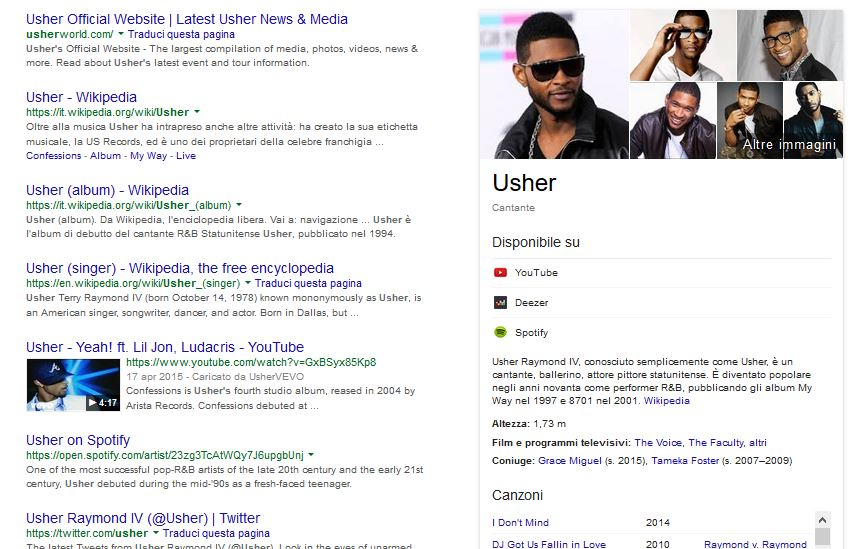
\includegraphics[width=\textwidth]{images/LInformazioneEIlWebSemantico-IlCasoUsher}
				\caption{Il web semantico - Informazione strutturata (sulla destra) raccolta tramite \emph{lifting}}
				\label{fig:LInformazioneEIlWebSemantico-IlCasoUsher}
			\end{figure}
			
		
		\subsection{Connettere le informazioni}
			Abbiamo visto le immense potenzialità che derivano dal \emph{lifting} dei dati, ma come è possibile fare questo? Di seguito spieghiamo un tipo di algoritmo adottato da Google che permette questa magia.
		
			\subsubsection{Scegliere i punti}
				Scegliere i punti si rivela il vero problema. Infatti i punti tra cui scegliere sono la radice quadrata della dimensione dei dati. La complessità quindi risulta:
				\[
					O(|E| \cdot |G_1|) + O(|G_1| \cdot |G_2|) = O((|E| + |G_2|) \cdot |G1|)
				\]
				Siamo partiti da con una complessità pari a $O(|G_1|\cdot|G_2|)$ con la tecnica \emph{brute force} e siamo arrivati a $O((|E| + |G_2|) \cdot |G1|)$. Abbiamo ottenuto un algoritmo peggiore ma non nella pratica, perché questo algoritmo messo in pratica funziona splendidamente e consente di avere un risparmio di costo computazionale del 95\% rispetto al \emph{brute force}.
			
			\subsubsection{Esporre i dati}
				Per esporre i dati nel web abbiamo diversi modi. Uno può essere quello di mostrare i dati come file sotto un URI, ma questo è poco pratico. Nella pratica si preferisce ricorrere a interfacce con cui fare \emph{query} usando SPARQL, offrendo in questo modo un servizio web molto potente e flessibile. Questi \emph{query} fatte attraverso indirizzo web con classici \emph{"urlencoding"} e passaggio parametri con GET HTTP sono chiamate \textbf{\emph{endpoint}}. Un esempio di SPARQL \emph{endpoint}:
				\begin{quote}
				\begin{verbatim}
					PREFIX dc <http://purl.org/dc/elements/1.1/>
					SELECT ?book ?who
					WHERE ( ?book dc:creator ?who )
				\end{verbatim}
				\end{quote}
				Un esempio concreto di un tale servizio è \href{http://wiki.dbpedia.org/}{dbpedia.com} da cui è possibile effettuare \emph{query} SPARQL e ottenere pagine come questa: tutta la conoscenza di \href{http://dbpedia.org/page/Albert_Einstein}{Albert Einstain} in una pagina.
				Le ontologie principale sono date da \href{https://schema.org/}{schema.org}. Un altro sito interessante è \href{http://www.visualdataweb.org/relfinder.php}{www.visualdatamedia.org}, il quale mette a disposizione un servizio che permette di navigare il grafo delle conoscenza sulle parole date. 
					
					
					